
% #1 x, #2 y, #3 no, #4-6 text
\newcommand\nocswitchbuffertxt[5]{
    \draw (#1+0.2, #2 + 0.8) node[draw, thick, minimum width=2cm, minimum height=0.8cm, anchor=north, inner sep=0pt] (in#3) {#5};
    \draw (#1+0.2, #2 + 1.6) node[draw, thick, minimum width=2cm, minimum height=0.8cm, anchor=north, inner sep=0pt] (out#3) {#4};
    \draw[thick] ([xshift=0.04em]in#3.south west) -- ([xshift=0.04em, yshift=-1em]in#3.south west);
    \draw[thick] ([xshift=-0.04em]in#3.south east) -- ([xshift=-0.04em, yshift=-1em]in#3.south east);
}

\newcommand\fliplab[1]{
    \rotatebox{180}{#1}
}

% #1 x, #2 y, #3 color
\newcommand\flit[3]{
    \draw (#1,#2) node[draw, rectangle, fill=#3, inner sep=0pt, minimum width=0.5cm, minimum height=0.5cm] {};
}
% #1 color
\newcommand\fflit[1]{
    \begin{tikzpicture}
    \draw node[draw, rectangle, fill=#1, inner sep=0pt, minimum width=0.5cm, minimum height=0.5cm] {};
    \end{tikzpicture}
}
    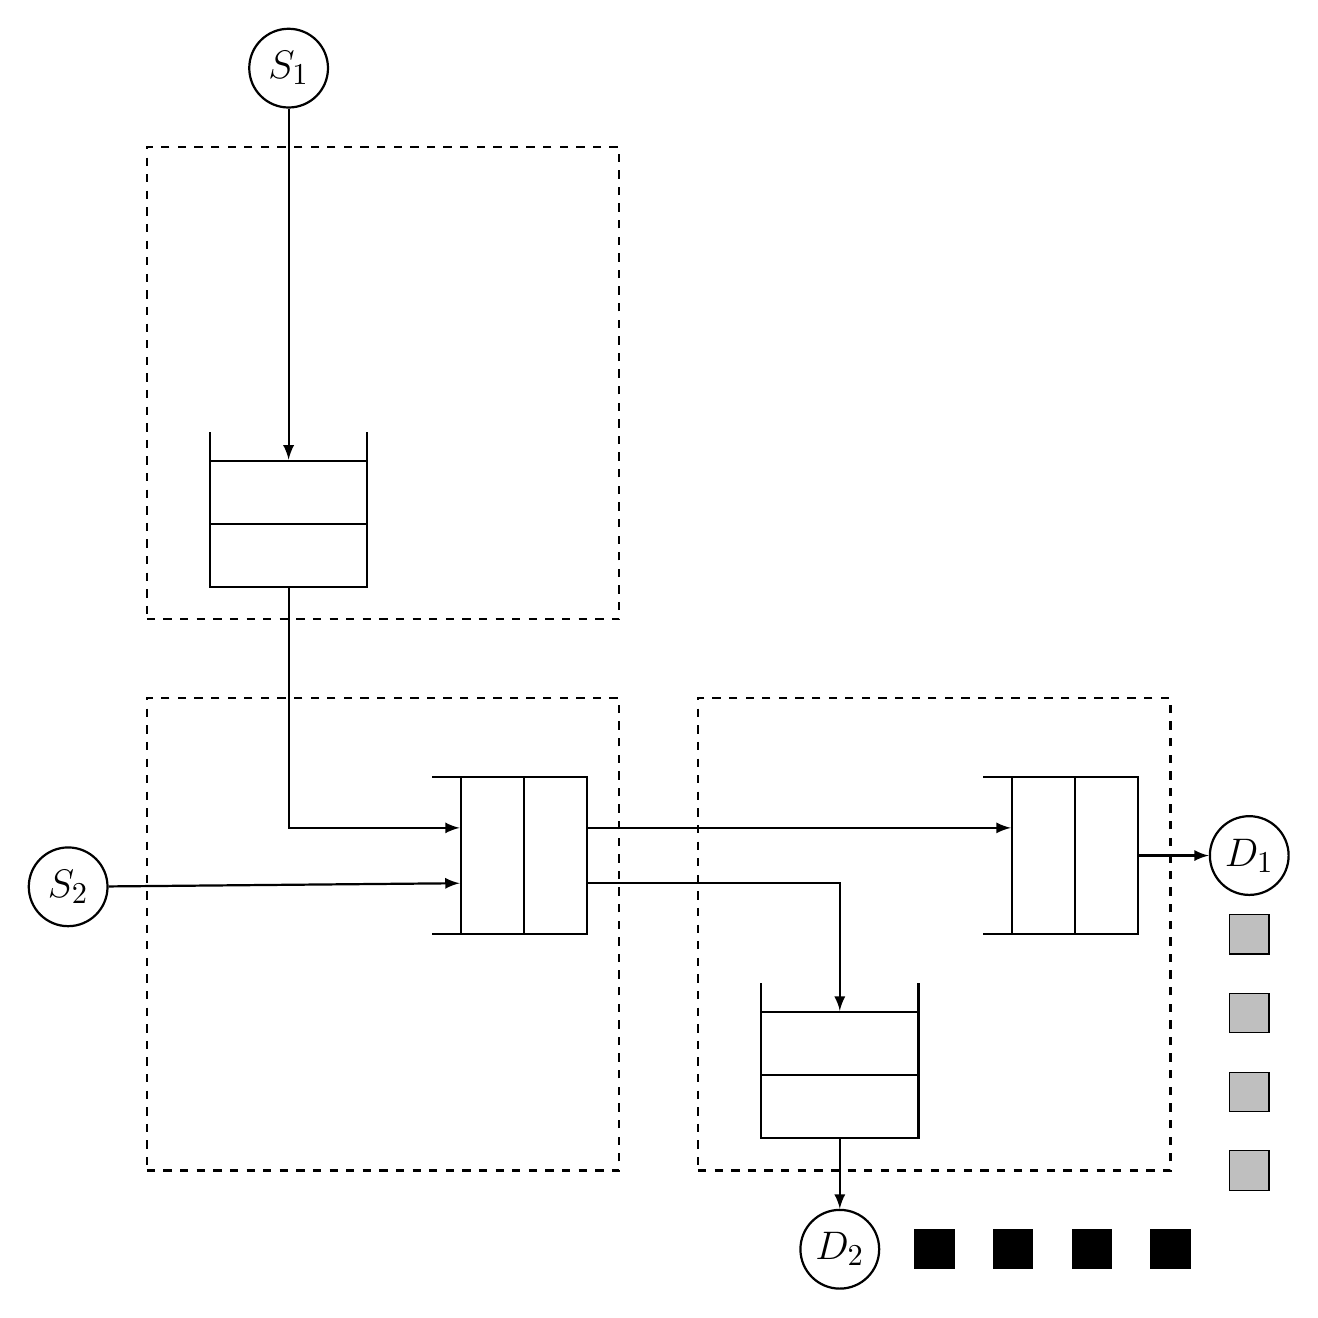
\begin{tikzpicture}[font={\fontsize{15pt}{12}\selectfont}]

    
    
        %\draw (-4.5,-6.5) node[draw, rectangle, thick, dashed, inner sep=0pt, anchor= south west, minimum width=18cm, minimum height=18cm] {};
    
    \draw (-3,-0.397) node[draw, circle, thick, inner sep=0pt, minimum size=1cm] (S2) {$S_2$};
    \draw (-0.2,10) node[draw, circle, thick, inner sep=0pt, minimum size=1cm] (S1) {$S_1$};
    \draw (12,0) node[draw, circle, thick, inner sep=0pt, minimum size=1cm] (D1) {$D_1$};
    \draw (6.8,-5) node[draw, circle, thick, inner sep=0pt, minimum size=1cm] (D2) {$D_2$};

        
        \flit{8}{-5}{black}
        \flit{9}{-5}{black}
        \flit{10}{-5}{black}
        \flit{11}{-5}{black}
        
        \flit{12}{-1}{lightgray}
        \flit{12}{-2}{lightgray}
        \flit{12}{-3}{lightgray}
        \flit{12}{-4}{lightgray}
 
    \draw (1,-1) node[draw, rectangle, thick, dashed, inner sep=0pt, minimum width=6cm, minimum height=6cm] {};
\begin{scope}[rotate=-90, transform shape]
    \nocswitchbuffertxt{-0.2}{2}{EB}{ }{  }
\end{scope}

\draw (1,6) node[draw, rectangle, thick, dashed, inner sep=0pt, minimum width=6cm, minimum height=6cm] {};
\begin{scope}[rotate=180, transform shape]
\nocswitchbuffertxt{0}{-5}{SA}{ }{  }
\end{scope}

 \draw (8,-1) node[draw, rectangle, thick, dashed, inner sep=0pt, minimum width=6cm, minimum height=6cm] {};
\begin{scope}[rotate=-90, transform shape]
    \nocswitchbuffertxt{-0.2}{9}{EC}{ }{  }
\end{scope}
\begin{scope}[rotate=180, transform shape]
    \nocswitchbuffertxt{-7}{2}{SC}{  }{  }
\end{scope}

    \draw[thick, -latex] (outSA) |- ([yshift=1em]inEB.south);
    \draw[thick, -latex] ([yshift=1em]outEB.north) -- ([yshift=1em]inEC.south);
    \draw[thick, -latex] ([yshift=-1em]outEB.north) -| (inSC.south);
    \draw[thick, -latex] (S2) -- ([yshift=-1em]inEB.south);
    \draw[thick, -latex] (outEC.north) -- (D1);
    \draw[thick, -latex] (outSC.north) -- (D2);
    \draw[thick, -latex] (S1) -- (inSA.south);
 
\end{tikzpicture}
